\section{Профиль и протокол}
\subsection{Цель и основные формулы}
Цель --- обучить полезное представление без меток, измерить влияние аугментаций и зависимость качества от числа доступных меток~\cite{teacher}. Два независимых преобразования $t_1,t_2\sim T$ одного изображения образуют положительную пару. ResNet-18 для CIFAR с первой свёрткой $3\times3$ без max-pool выдаёт $h\in\mathbb R^{512}$. Голова без bias $512\to512\to128$ с ReLU строит $z$, затем $\hat z=z/\|z\|_2$.
\begin{equation}\ell_i=-\log\frac{\exp(\hat z_i^\top\hat z_{j(i)}/\tau)}{\sum_{k\ne i}\exp(\hat z_i^\top\hat z_k/\tau)},\qquad \mathcal L=\frac1{2N}\sum_{i=1}^{2N}\ell_i.\end{equation}
У каждого вида один положительный и $2N-2$ отрицательных примера. Самосходство исключается. При равных сходствах $\mathcal L=\ln(2N-1)$. Температура меняет концентрацию весов $p_{ik}\propto\exp(s_{ik}/\tau)$ и масштаб градиента $1/\tau$: сильнее отталкиваются наиболее похожие отрицательные примеры.

Для ковариации $C$ с собственными значениями $\lambda_j$ эффективный ранг равен
\begin{equation}q_j=\lambda_j/\operatorname{tr}C,\qquad r_{eff}=\exp\left(-\sum_jq_j\ln q_j\right).\end{equation}
При $\operatorname{tr}C\le10^{-6}d\,\overline{\|h\|^2}$ ранг не определён и помечается как n/a. Малый $r_{eff}/d<0.2$ --- диагностика размерностного коллапса, а не доказательство отсутствия классовой информации. Полное совпадение нормированных проекций даёт $\|\bar{\hat z}\|=1$.

\subsection{Данные и обучение}
Профиль: $\tau=0.1$, третья операция flip, доли меток $r=0.02,0.05,0.25,1$. CIFAR-10: train 43 000, val 5000, cal 2000, test 10 000; статистики нормализации рассчитаны на train. Предобучение использует только изображения train, cal не читается. Базовый набор $T$: RandomResizedCrop $32\times32$, scale $[0.08,1]$; ColorJitter с вероятностью 0.8, brightness/contrast/saturation 0.4 и hue 0.1; flip с вероятностью 0.5. Генератор видов независим от split и инициализации.

SimCLR: SGD, LR 0.3, momentum 0.9, weight decay $10^{-4}$, cosine с прогревом 10 эпох, $N=256$, полное обучение 100 эпох, короткое 25. Одновременно обрабатываются 512 видов и 510 отрицательных примеров для каждого; AMP используется для сети, NT-Xent считается в float32. Устройство --- RTX 3060 Laptop. B0 не обучается; B1 обучен с учителем на всех train-метках за 25 эпох с crop и flip.

Кодировщик и BatchNorm заморожены в eval. Признаки извлечены без аугментаций. Probe --- линейный классификатор, 200 эпох, LR 0.1; регуляризация выбирается по val из $0,0.001,0.01$. kNN использует только train, $k=200$, температура 0.07. Во всех условиях одинаковая процедура оценки.
\begin{figure}[H]\centering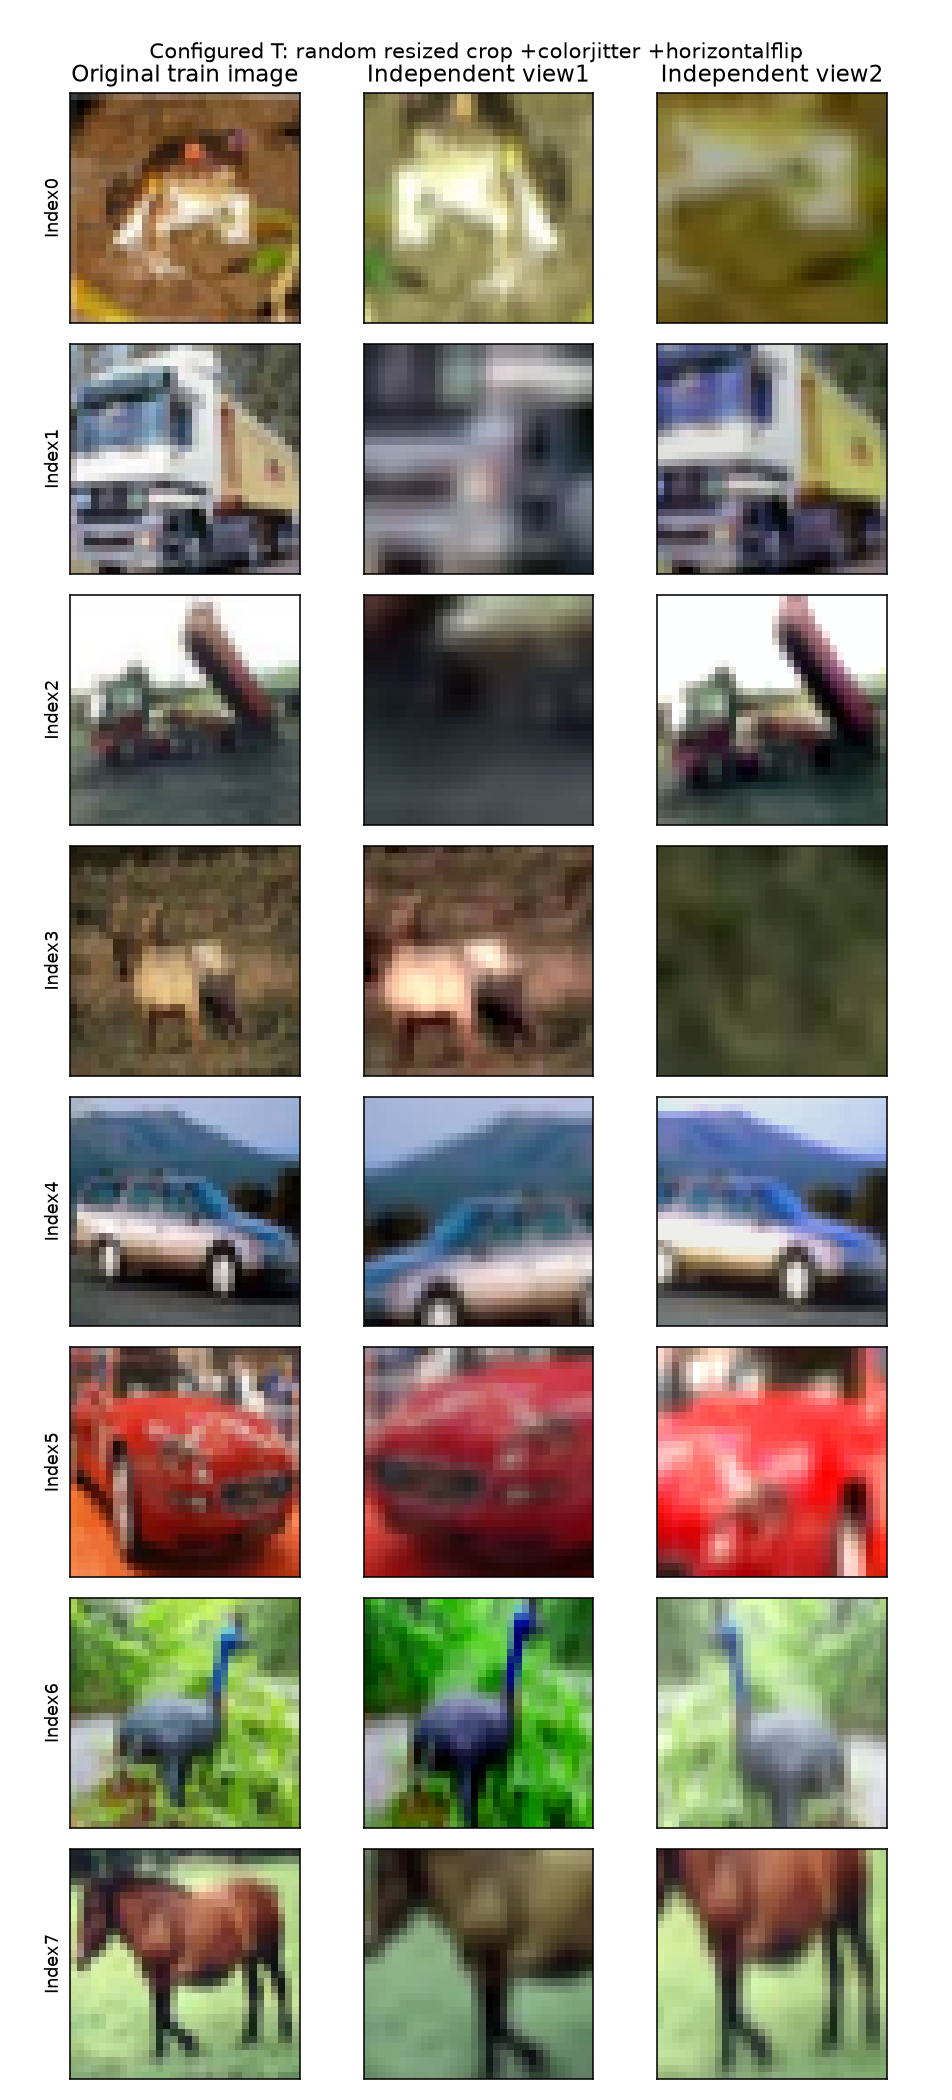
\includegraphics[width=\linewidth,height=.38\textheight,keepaspectratio]{figures/views.png}
\caption{Восемь исходных изображений train и независимые виды базового набора.}\label{fig:views}
\end{figure}

\section{E1. SimCLR и базовые модели}
Ожидалось преимущество SimCLR над случайным кодировщиком, но не обязательное равенство модели с учителем. Оценка probe проведена в пяти точках, включая начальную.
\begin{table}[H]\centering\footnotesize
\setlength{\tabcolsep}{4pt}
\caption{Три фиксированных кодировщика E1: качество на test и диагностика на train.}\label{tab:e1}
\begin{tabular}{lrrrrrrl}
\toprule
Модель & Probe & kNN & $\operatorname{tr}C_h$ & $r_{eff,h}$ & $r_{eff,h}/512$ & $\|\bar{\hat z}\|$ & Ист. \\
\midrule
B0 & 0.4357 & 0.3822 & 95.464 & 3.156 & 0.0062 & 0.9932 & R01 \\
B1 & 0.8988 & 0.8959 & 34.552 & 16.492 & 0.0322 & 0.7673 & R02 \\
SimCLR & 0.7662 & 0.7053 & 8.283 & 75.610 & 0.1477 & 0.0398 & R03 \\
\bottomrule
\end{tabular}
\end{table}


\begin{table}[H]\centering\small
\setlength{\tabcolsep}{4pt}
\caption{Масштаб и ранг признаков на 5000 фиксированных train-изображений.}\label{tab:diagnostics}
\begin{tabular}{llrrrr}
\toprule
Модель & Признак & $d$ & $\overline{\|h\|}$ & $\operatorname{tr}C$ & $r_{eff}$ \\
\midrule
B0 & $h$ & 512 & 35.5166 & 95.46421 & 3.156 \\
B0 & $\hat z$ & 128 & 1.0000 & 0.01348 & 28.474 \\
B1 & $h$ & 512 & 7.6857 & 34.55226 & 16.492 \\
B1 & $\hat z$ & 128 & 1.0000 & 0.41126 & 19.099 \\
SimCLR & $h$ & 512 & 3.5061 & 8.28280 & 75.610 \\
SimCLR & $\hat z$ & 128 & 1.0000 & 0.99862 & 59.873 \\
\bottomrule
\end{tabular}
\end{table}


\begin{table}[H]\centering\small
\setlength{\tabcolsep}{4pt}
\caption{Probe в пяти контрольных точках одного обучения SimCLR.}\label{tab:checkpoints}
\begin{tabular}{rrrrrl}
\toprule
Эпоха & Test acc. & Val acc. & $r_{eff,h}$ & $r_{eff,z}$ & Ист. \\
\midrule
0 & 0.4357 & 0.4302 & 3.156 & 28.474 & R04 \\
25 & 0.6769 & 0.6862 & 44.777 & 38.427 & R05 \\
50 & 0.7211 & 0.7366 & 56.931 & 49.145 & R06 \\
75 & 0.7529 & 0.7532 & 68.379 & 56.541 & R07 \\
100 & 0.7662 & 0.7616 & 75.610 & 59.873 & R03 \\
\bottomrule
\end{tabular}
\end{table}


Итоговый средний loss по эпохе равен 0.553783, ниже $\ln511=6.236370$. Выигрыш над B0 на полной разметке $G(1)=0.7662-0.4357=0.3305$; отставание от B1 равно 0.1326. Это разные бюджеты supervision, а не чистая цена отказа от меток.
\begin{figure}[H]\centering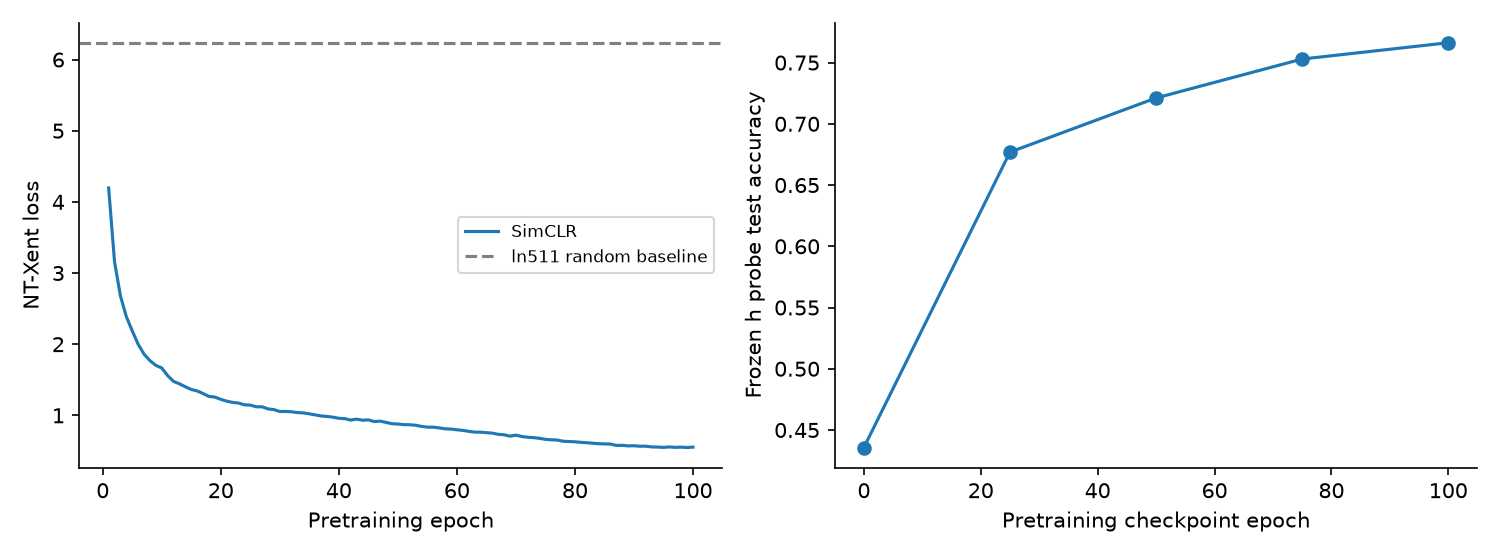
\includegraphics[width=\linewidth,height=.35\textheight,keepaspectratio]{figures/loss.png}
\caption{E1: NT-Xent, случайный уровень и probe по эпохам.}\label{fig:loss}
\end{figure}

\begin{figure}[H]\centering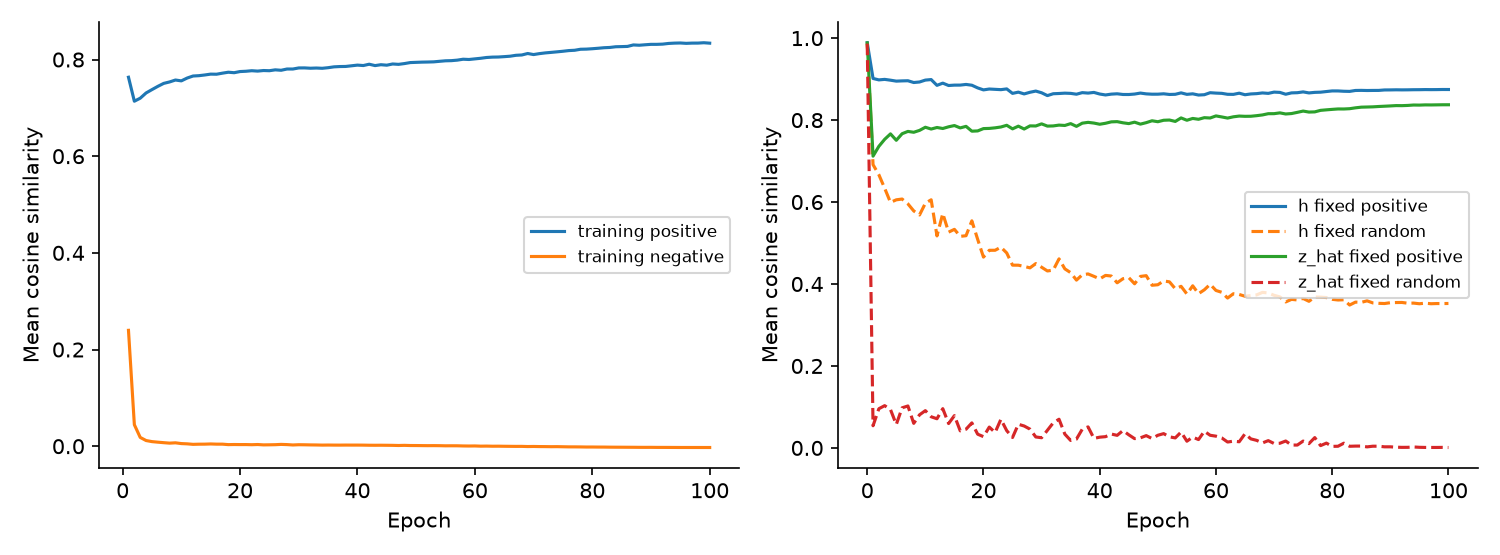
\includegraphics[width=\linewidth,height=.32\textheight,keepaspectratio]{figures/similarity.png}
\caption{Сходства положительных и случайных пар по эпохам.}\label{fig:similarity}
\end{figure}

\begin{figure}[H]\centering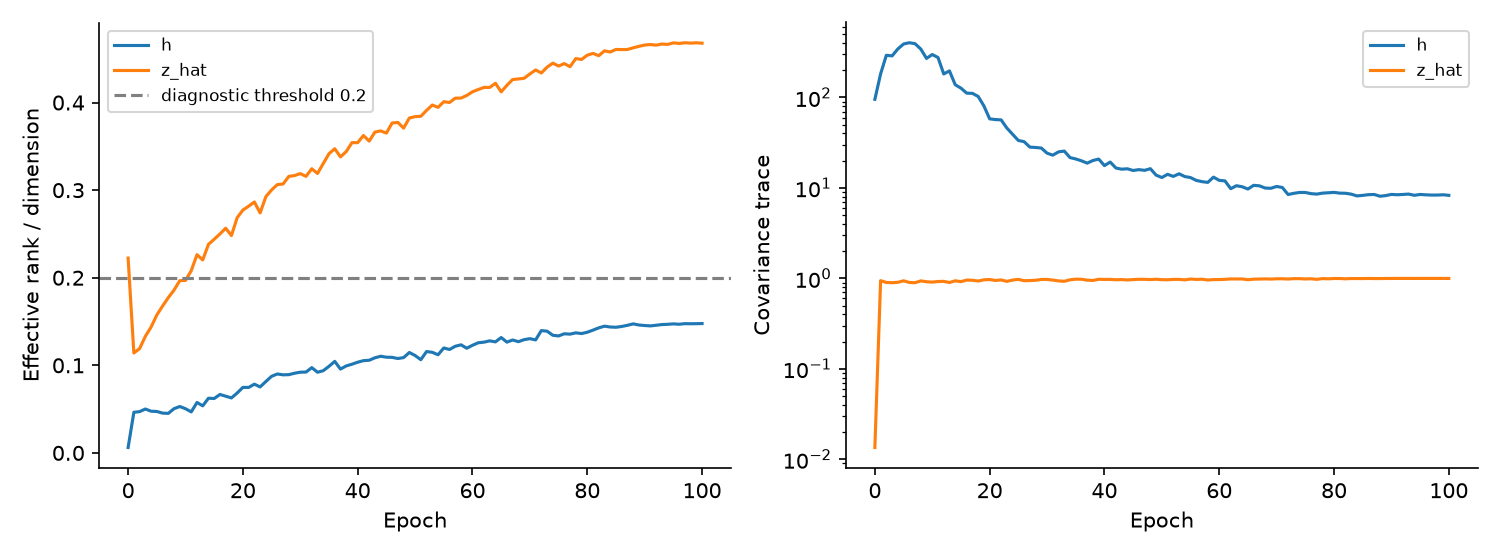
\includegraphics[width=\linewidth,height=.37\textheight,keepaspectratio]{figures/rank.png}
\caption{Эффективный ранг и след ковариации по эпохам.}\label{fig:rank}
\end{figure}

\begin{figure}[H]\centering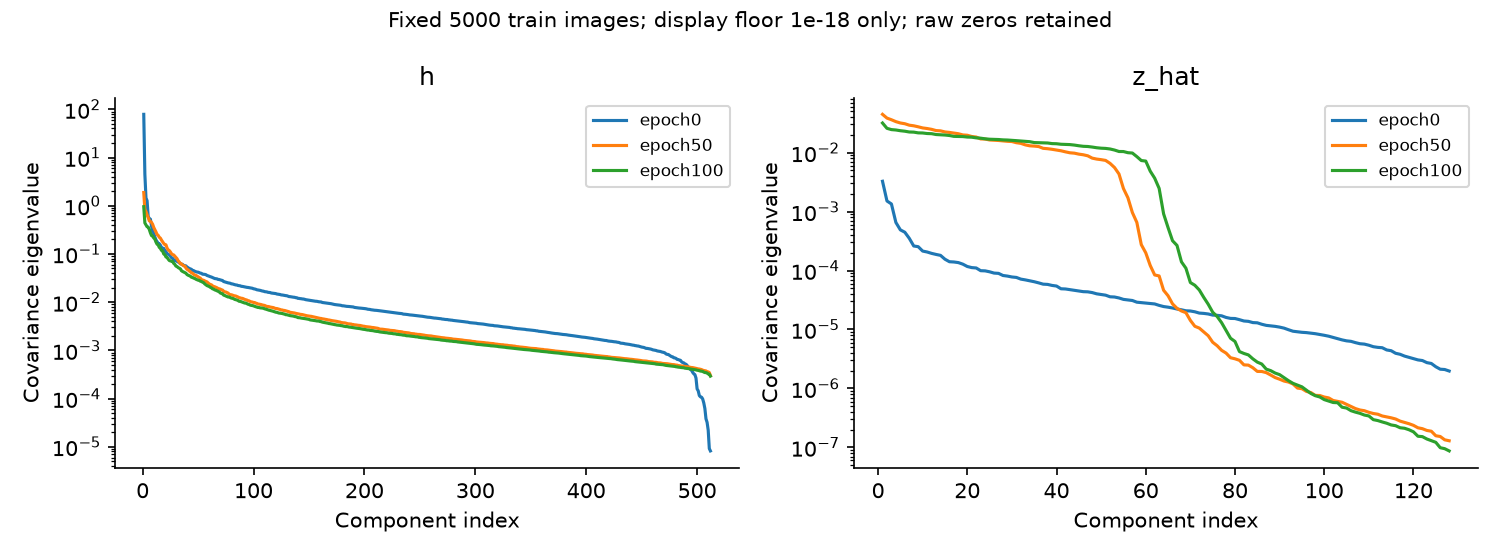
\includegraphics[width=\linewidth,height=.37\textheight,keepaspectratio]{figures/spectra.png}
\caption{Спектры ковариации в начале, середине и конце обучения.}\label{fig:spectra}
\end{figure}

От 25 к 50 эпохам loss снизился на 0.265433, probe вырос на 0.0442; от 50 к 75 --- на 0.215363 и 0.0318; от 75 к 100 --- на 0.109146 и 0.0133. Рост качества замедляется. На измеренных соседних точках строгого плато с изменением accuracy не более 0.01 при падении loss не менее 0.05 не обнаружено. Нельзя приписывать данным отсутствующее плато.

У всех трёх кодировщиков $r_{eff,h}/512<0.2$, однако классификация различается сильно. У SimCLR нормированные проекции хорошо разнесены ($\|\bar{\hat z}\|=0.039754$), их ранг 59.873 из 128 и след 0.998619. Таким образом, диагностический низкий ранг $h$ сосуществует с полезным представлением и не равен полному коллапсу.

\section{E2. Вклад аугментаций}
Шесть коротких обучений имеют общий seed 1, архитектуру, batch, $\tau$ и оптимизацию; меняется только набор операций. $\Delta_j=M(T)-M(T_{-j})$. Для короткого полного набора $G_0=0.6691-0.4357=0.2334$, половина выигрыша 0.1167.
\begin{table}[H]\centering\footnotesize
\setlength{\tabcolsep}{4pt}
\caption{E2: 25 эпох, один seed; положительная разность означает пользу удалённой операции.}\label{tab:e2}
\begin{tabular}{lrrrrrl}
\toprule
Вариант & Probe & kNN & $\Delta_j$ & $r_{eff,h}/512$ & $\|\bar{\hat z}\|$ & Ист. \\
\midrule
T & 0.6691 & 0.5967 & +0.0000 & 0.0718 & 0.0339 & R08 \\
без crop & 0.3889 & 0.3457 & +0.2802 & 0.0682 & 0.0171 & R09 \\
без color & 0.5599 & 0.4863 & +0.1092 & 0.0811 & 0.0396 & R10 \\
без flip & 0.6862 & 0.6083 & -0.0171 & 0.0718 & 0.0378 & R11 \\
только crop & 0.5599 & 0.4806 & +0.1092 & 0.0805 & 0.0408 & R12 \\
без операций & 0.3614 & 0.3304 & +0.3077 & 0.0931 & 0.0175 & R13 \\
\bottomrule
\end{tabular}
\end{table}


\begin{figure}[H]\centering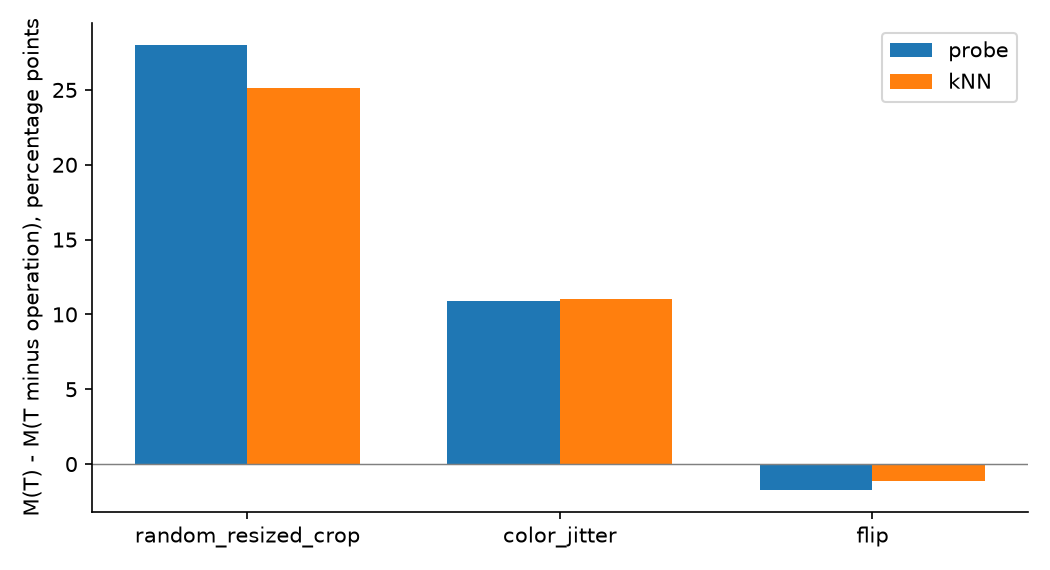
\includegraphics[width=\linewidth,height=.32\textheight,keepaspectratio]{figures/ablation.png}
\caption{Вклад каждой из трёх операций в probe и kNN.}\label{fig:ablation}
\end{figure}

Crop задаёт устойчивость к положению, масштабу и частичной видимости. Его удаление уменьшило probe на 0.2802, что превышает половину выигрыша: операция критична и по качеству. ColorJitter задаёт устойчивость к яркости, контрасту, насыщенности и оттенку; падение 0.1092 ниже половины выигрыша. Flip задаёт устойчивость к горизонтальному отражению; удаление повысило accuracy на 0.0171, но этого недостаточно для вывода о вреде.

Во всех вариантах, включая полный $T$, присутствует диагностический низкий ранг $h$. Поэтому формальная коллапсная ветвь правила задания помечает удаления как критичные; она не доказывает нового коллапса из-за удаления. Это ограничение отделено от изменения accuracy. По одному seed малые эффекты не считаются установленными.
\begin{figure}[H]\centering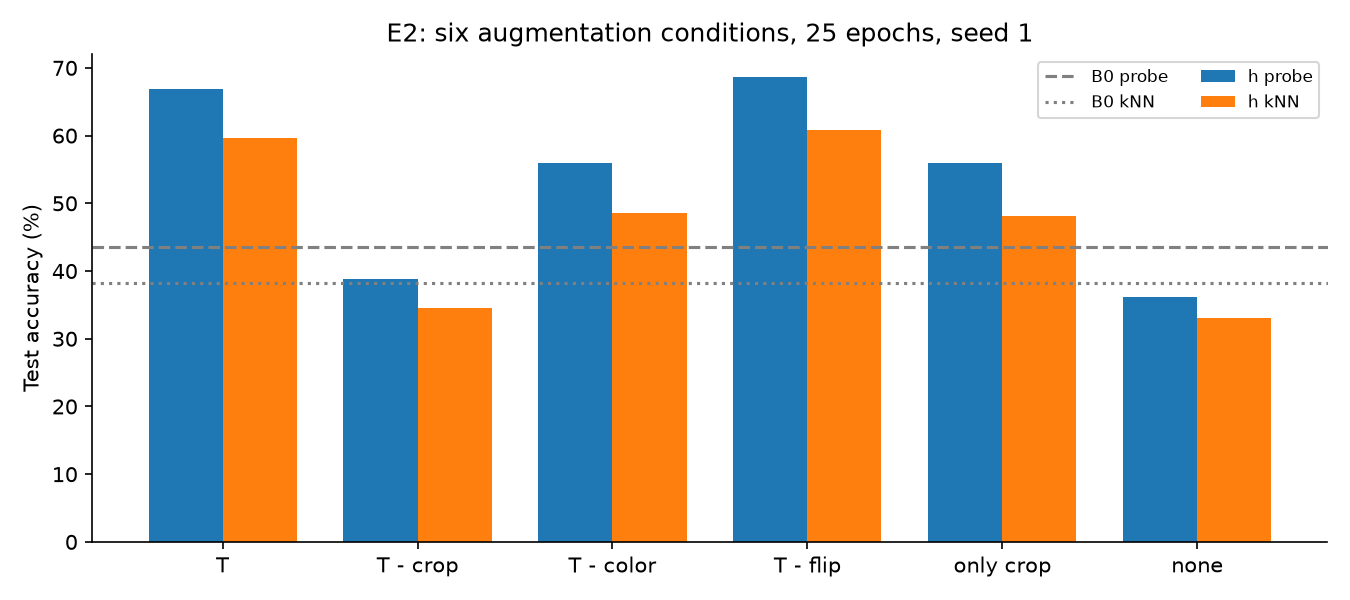
\includegraphics[width=\linewidth,height=.32\textheight,keepaspectratio]{figures/variants.png}
\caption{Шесть вариантов E2, включая одну операцию и совпадающие виды.}\label{fig:variants}
\end{figure}

Из одиночных операций оставлен crop, выбранный по максимальному $\Delta_j$; accuracy 0.5599. Совпадающие виды без операций дали 0.3614, ниже B0 0.4357, при $\|\bar{\hat z}\|=0.017496$. Следовательно, плохое качество здесь не связано с совпадением всех проекций. При одинаковых видах притяжение пары почти не требует инвариантности, а отталкивание продолжает различать отдельные изображения; такая геометрия не обязана разделять классы.

\section{E3. Эффективность по меткам}
Используются одни сохранённые кодировщики E1. Общие seed 1,2,3 меняют стратифицированные вложенные подмножества меток и инициализацию probe. Число меток: 860, 2150, 10 750 и 43 000. Основное сравнение --- SimCLR минус B0 при $r_{min}=0.02$; все остальные условия фиксированы. До запусков предсказан положительный эффект величины 0.165250; отсутствие устойчивого положительного различия опровергло бы направленный прогноз.
\begin{table}[H]\centering\footnotesize
\setlength{\tabcolsep}{4pt}
\caption{Полная матрица E3: точность всех трёх кодировщиков при каждой доле и seed.}\label{tab:matrix}
\begin{tabular}{rrrrrl}
\toprule
$r$ & Seed & B0 & B1 & SimCLR & Источники \\
\midrule
0.02 & 1 & 0.2903 & 0.8792 & 0.6644 & R14/R15/R16 \\
0.02 & 2 & 0.2882 & 0.8817 & 0.6652 & R17/R18/R19 \\
0.02 & 3 & 0.2922 & 0.8795 & 0.6599 & R20/R21/R22 \\
0.05 & 1 & 0.3404 & 0.8871 & 0.7009 & R23/R24/R25 \\
0.05 & 2 & 0.3489 & 0.8900 & 0.7097 & R26/R27/R28 \\
0.05 & 3 & 0.3400 & 0.8910 & 0.7037 & R29/R30/R31 \\
0.25 & 1 & 0.4142 & 0.8964 & 0.7491 & R32/R33/R34 \\
0.25 & 2 & 0.4108 & 0.8978 & 0.7483 & R35/R36/R37 \\
0.25 & 3 & 0.4093 & 0.8978 & 0.7494 & R38/R39/R40 \\
1.0 & 1 & 0.4357 & 0.8988 & 0.7662 & R01/R02/R03 \\
1.0 & 2 & 0.4380 & 0.8997 & 0.7647 & R41/R42/R43 \\
1.0 & 3 & 0.4385 & 0.8984 & 0.7641 & R44/R45/R46 \\
\bottomrule
\end{tabular}
\end{table}


\begin{table}[H]\centering\small
\setlength{\tabcolsep}{4pt}
\caption{Парные разности SimCLR минус B0, выборочное SD и критерий задания.}\label{tab:gains}
\begin{tabular}{rrrrrr}
\toprule
$r$ & $\Delta_1$ & $\Delta_2$ & $\Delta_3$ & $\bar\Delta$ & $s_\Delta$ \\
\midrule
0.02 & +0.3741 & +0.3770 & +0.3677 & 0.372933 & 0.004759 \\
0.05 & +0.3605 & +0.3608 & +0.3637 & 0.361667 & 0.001767 \\
0.25 & +0.3349 & +0.3375 & +0.3401 & 0.337500 & 0.002600 \\
1.0 & +0.3305 & +0.3267 & +0.3256 & 0.327600 & 0.002571 \\
\bottomrule
\end{tabular}
\end{table}


\begin{figure}[H]\centering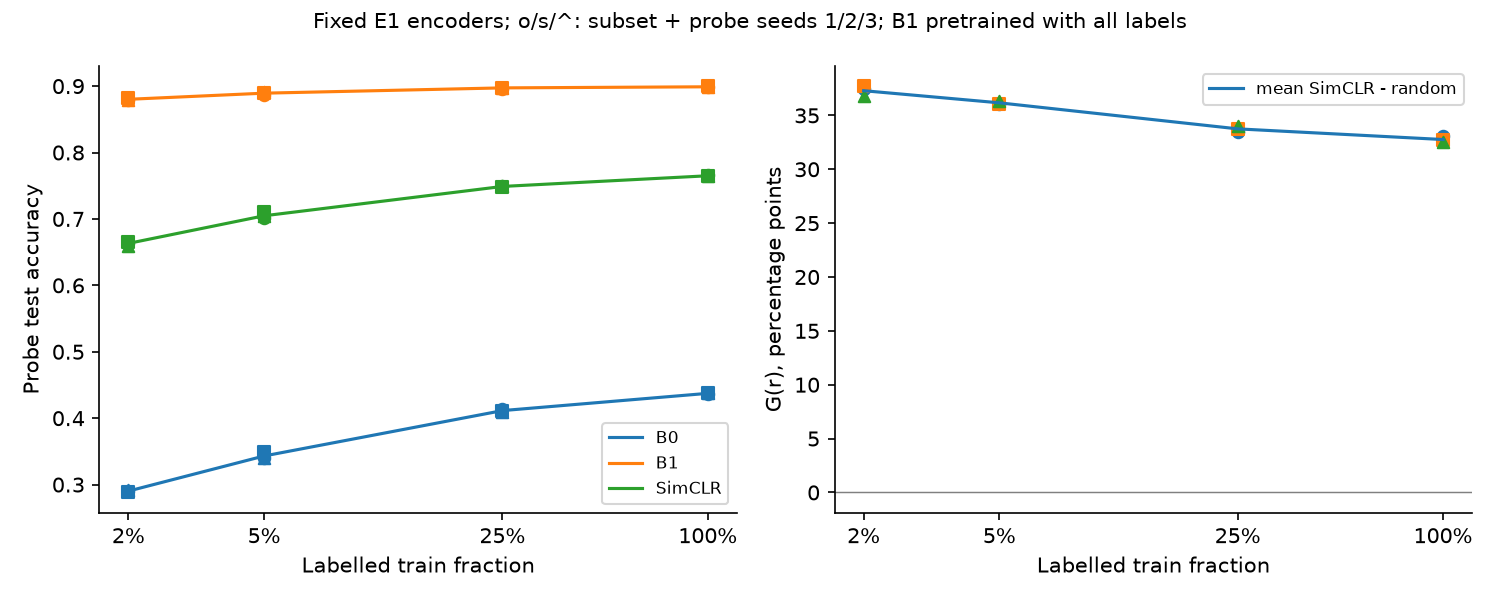
\includegraphics[width=\linewidth,height=.40\textheight,keepaspectratio]{figures/efficiency.png}
\caption{E3: все seed по долям разметки и выигрыш SimCLR над B0.}\label{fig:efficiency}
\end{figure}

При $r_{min}$ все разности положительны: 0.3741, 0.3770, 0.3677. Среднее 0.372933, выборочное SD 0.004759; $\bar\Delta>2s_\Delta=0.009517$. Различие установлено в пользу SimCLR. Направление гипотезы поддержано, но точечный прогноз ошибся на +0.207683: количественное ожидание было слишком консервативным. При $r=1$ средний выигрыш 0.327600 также установлен. Три оценки seed 1 на полном train явно повторно используют E1.

\section{Ответы на контрфактические вопросы}
\subsection*{Вопрос 1. Сравнимость NT-Xent}
В полном E1 первый и последний шаг дали 6.110858 и 0.597880, при случайном уровне 6.236370 (R47). Для $N=256$, 25 эпох: 6.110858 $\to$ 1.034946 (R48). Для $N=64$, 25 эпох: 4.693625 $\to$ 0.495635 при $\ln127=4.844187$ (R49). Величины loss зависят от числа кандидатов и температуры. При изменении batch также меняются число обновлений и статистики BatchNorm, поэтому это не изолированная проверка одного знаменателя.

\subsection*{Вопрос 2. Класс, определяемый оттенком}
Построен HueCIFAR-10: исходные train/val/test 43\,000/5\,000/10\,000 изображений сохраняют роли, cal не читается. Семантические метки отброшены. В каждой роли случайно и точно поровну назначены десять классов оттенка, независимо от содержания, с seed 4601/4602/4603. Для класса k оттенок равен $(k+0.5)/10+u$, $u\sim U[-0.015,0.015]$, насыщенность 0.8; яркость $V=0.25+0.65(0.299R+0.587G+0.114B)$. HSV переведён в RGB с округлением до uint8. Текстура яркости сохраняется, класс задаётся только оттенком.

Использованы два уже обученных 25 эпох кодировщика E2: полный T и вариант без ColorJitter. Предобучение не повторялось, кодировщики и BatchNorm заморожены. На h обучены линейные пробы: 200 эпох, SGD 0.1, momentum 0.9, cosine, seed 1. L2 выбирается из $\{0,0.001,0.01\}$ по val; признаки стандартизуются только по train. До обучения ожидалось преимущество варианта без изменения цвета.
\begin{table}[H]\centering\small
\setlength{\tabcolsep}{4pt}
\caption{Цветовой контроль: два замороженных кодировщика E2, один seed и одинаковый probe.}\label{tab:hue_control}
\begin{tabular}{lrrrl}
\toprule
Кодировщик & L2 & Val accuracy & Test accuracy & Ист. \\
\midrule
T & 0.001 & 0.991800 & 0.994000 & C1 \\
$T_{-ColorJitter}$ & 0.000 & 0.999800 & 0.999700 & C2 \\
\bottomrule
\end{tabular}
\end{table}


\begin{figure}[H]\centering
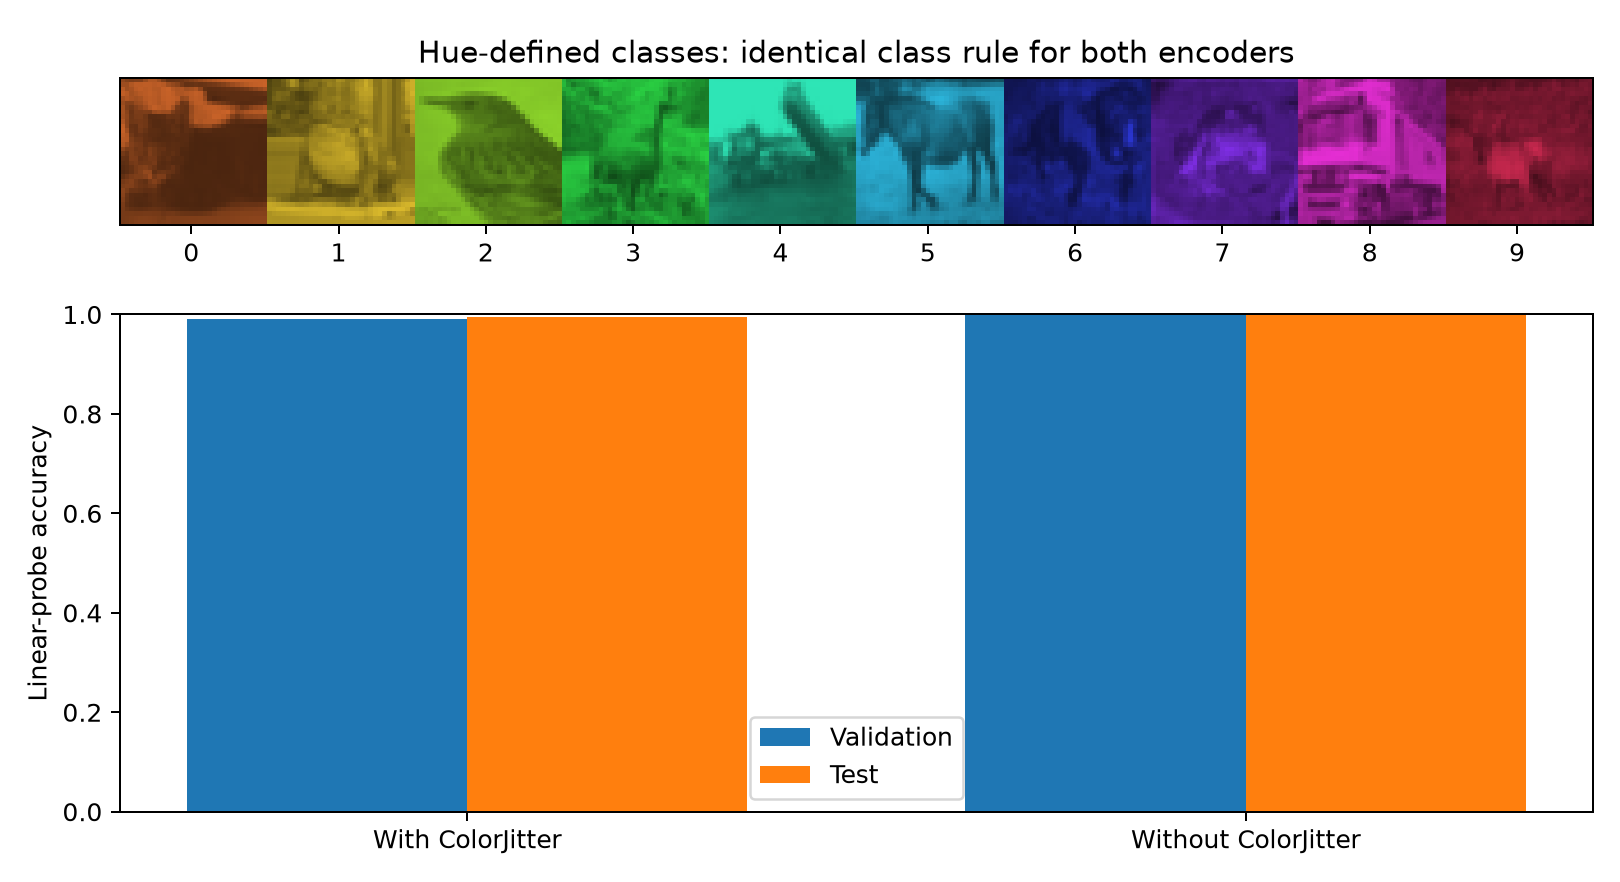
\includegraphics[width=\linewidth]{figures/hue_control.png}
\caption{Примеры классов по оттенку и точность линейных проб на цветовой задаче.}
\end{figure}
Точность без ColorJitter выше; разность test accuracy «без минус с» равна +0.005700. Предсказанное направление подтверждено в этом контроле.
Это прямой контроль информации об оттенке в h при данных кодировщиках. Один seed не устанавливает устойчивость разности; результат не переносится автоматически на классификацию CIFAR по предметным классам и не означает полного удаления цвета проекционной головой.
\subsection*{Вопрос 3. Ранг и полезность}
SimCLR на эпохе 25 имеет $r_{eff,h}=44.7773$, probe 0.6769 (R05); E2 без ColorJitter --- 41.4983 и 0.5599. Ранг отличается примерно на 7.3\%, accuracy --- на 0.1170. Напротив, полный короткий $T$ имеет ранг 36.7625 и accuracy 0.6691: accuracy близка (разрыв 0.0078), ранг отличается на 17.9\%. Ранг измеряет распределение дисперсии, а не ориентацию относительно классов. При исчезающем следе ковариации вопрос о ранге теряет смысл по принятой конвенции.
\subsection*{Вопрос 4. Голова и признаки}
Probe на $h$ даёт 0.7662, на $\hat z$ --- 0.6820, разность +0.0842; kNN соответственно 0.7053 и 0.7352 (R50). Проекционная голова меняет размерность и геометрию, усиливает заданные аугментациями инвариантности и может отбросить полезные для линейного классификатора сведения. Это не означает вреда головы для самого контрастного обучения или всех downstream-задач.
\subsection*{Вопрос 5. Выигрыш и бюджет supervision}
$G(r_{min})=0.372933$ больше $G(1)=0.327600$ на 0.045333. Исходный B1 уже видел 43 000 train-меток, даже если probe видит только 860. Поэтому $M_{B1}(r)-M_{SSL}(r)$ не является ценой отказа от меток. Сохранённый контроль B1 обучен только на тех же 860 индексах: accuracy 0.4155 (R51), против 0.8792 для исходного B1 и 0.6644 для SSL при seed 1. Однако за 25 эпох low-label модель сделала 100 обновлений против 4200 у полного B1; SSL видел все 43 000 изображений без меток за 100 эпох. Бюджеты exposure и вычислений остаются разными.

\section{Ограничения и заключение}
Seed E3 не меняет предобучение: вывод относится к одному кодировщику SimCLR. Для выбора регуляризации используются 5000 размеченных val-изображений, что делает малую разметку train идеализированной. E2 исследует 25 эпох и один seed; эффекты не равны итогам 100 эпох. Цветовой контроль использует один seed и замороженные кодировщики; его область применимости отделена от предметных классов CIFAR.

SimCLR улучшил качество над случайными признаками и сохранил преимущество при малой разметке. Crop оказался наиболее существенной операцией по accuracy. Loss, эффективный ранг и downstream-качество описывают разные свойства: ни один из первых двух показателей не заменяет оценку probe и kNN.
\clearpage
\renewcommand{\refname}{Список использованных источников}
\begin{thebibliography}{9}
\addcontentsline{toc}{section}{Список использованных источников}
\bibitem{teacher} Лабораторная работа 4. Self-Supervised Representation Learning. Contrastive learning, invariances, collapse diagnostics и label efficiency. Курс «Нейронные сети». Методические указания, 2026.
\end{thebibliography}
\clearpage
\section*{Приложение. Идентификация запусков}
\addcontentsline{toc}{section}{Приложение. Идентификация запусков}
\begingroup\small\setstretch{1.05}
\begin{longtable}{@{}l>{\raggedright\arraybackslash}p{3.5cm}p{10.8cm}@{}}
\caption{Полные RUN\_ID источников результатов.}\\
\toprule Код & Условие & RUN\_ID \\ \midrule \endhead
\hypertarget{R01}{R01} & B0 full probe & {\fontsize{8.8}{11}\selectfont\texttt{20986de0ae364d2e58ce-02995bd34d574f009efb1948d5bbb2de}} \\
\hypertarget{R02}{R02} & B1 full probe & {\fontsize{8.8}{11}\selectfont\texttt{6772377c79bbe0439794-1c25b550be9d459ca96f4047f14051de}} \\
\hypertarget{R03}{R03} & SimCLR full probe & {\fontsize{8.8}{11}\selectfont\texttt{3ec66db45b2793e9a39a-1178fb68191d4a91813cdcb3596c91f8}} \\
\hypertarget{R04}{R04} & SSL epoch0 & {\fontsize{8.8}{11}\selectfont\texttt{32b6ee4ef289f8d231a3-6c65a07572794cae8e7d03d90aa20d21}} \\
\hypertarget{R05}{R05} & SSL epoch25 & {\fontsize{8.8}{11}\selectfont\texttt{161af2ac59fc30cca93c-a9707c14f765463591f3b0b35c51e615}} \\
\hypertarget{R06}{R06} & SSL epoch50 & {\fontsize{8.8}{11}\selectfont\texttt{814c55f620edc283039f-1d307201830645fbbb91b206ed96f1e6}} \\
\hypertarget{R07}{R07} & SSL epoch75 & {\fontsize{8.8}{11}\selectfont\texttt{b5657df9be0f7d211876-cb13a08b891d4512b26e0001d0fcf6e7}} \\
\hypertarget{R08}{R08} & E2 T & {\fontsize{8.8}{11}\selectfont\texttt{f6930c0a3a68eee5f646-633b0a71ee11487bbda64c3c2b30dfa7}} \\
\hypertarget{R09}{R09} & E2 без crop & {\fontsize{8.8}{11}\selectfont\texttt{e0d41b4aae60ede11d38-9215f50ca3ca44209c28a2caef62eb66}} \\
\hypertarget{R10}{R10} & E2 без color & {\fontsize{8.8}{11}\selectfont\texttt{03116a6d278a2596e1ac-5c320e06d35f4db9806cc7143980c9c6}} \\
\hypertarget{R11}{R11} & E2 без flip & {\fontsize{8.8}{11}\selectfont\texttt{1ba737be8226bf3d27f9-1aec3789ae7943b0a164c7f1b9bb01bc}} \\
\hypertarget{R12}{R12} & E2 только crop & {\fontsize{8.8}{11}\selectfont\texttt{76ffb8d4e5612d080fc6-81d66cafbc3f41f68510e06e129e17f9}} \\
\hypertarget{R13}{R13} & E2 без операций & {\fontsize{8.8}{11}\selectfont\texttt{11791a48092c8a621248-b32b5566845a44a98a747e62a041c408}} \\
\hypertarget{R14}{R14} & E3 B0 r0.02 s1 & {\fontsize{8.8}{11}\selectfont\texttt{3c7f8aef44b742e0d740-bd1161b222d74355b48b70233c125f00}} \\
\hypertarget{R15}{R15} & E3 B1 r0.02 s1 & {\fontsize{8.8}{11}\selectfont\texttt{bb3af5bd7af619070d74-06292b0f3b3c44dc81c24e0ab6d172f5}} \\
\hypertarget{R16}{R16} & E3 SimCLR r0.02 s1 & {\fontsize{8.8}{11}\selectfont\texttt{d0f2ed8844513313f79a-aecf0e05c9a149a99c35bef5fe93ebf2}} \\
\hypertarget{R17}{R17} & E3 B0 r0.02 s2 & {\fontsize{8.8}{11}\selectfont\texttt{0a61afbb48f9b3fe8fed-94f3228db806496986f85002bb6ee3af}} \\
\hypertarget{R18}{R18} & E3 B1 r0.02 s2 & {\fontsize{8.8}{11}\selectfont\texttt{44e30187926a9335ad65-a8df351b229f4891bab31aa621eac135}} \\
\hypertarget{R19}{R19} & E3 SimCLR r0.02 s2 & {\fontsize{8.8}{11}\selectfont\texttt{f2d962fdb04c1ea9c080-5310603d7990472cbd3f857b3a07b517}} \\
\hypertarget{R20}{R20} & E3 B0 r0.02 s3 & {\fontsize{8.8}{11}\selectfont\texttt{735bd7988fe54fb5ed5c-6638d16ec9d24dec8fdff3e1e412762a}} \\
\hypertarget{R21}{R21} & E3 B1 r0.02 s3 & {\fontsize{8.8}{11}\selectfont\texttt{7707b4c1b6abad188a76-fe2824b588b8432097b21ee1b7ff58f1}} \\
\hypertarget{R22}{R22} & E3 SimCLR r0.02 s3 & {\fontsize{8.8}{11}\selectfont\texttt{e80a6111230ce1625d1d-f62531a87cd0450a89b1cdc99080048f}} \\
\hypertarget{R23}{R23} & E3 B0 r0.05 s1 & {\fontsize{8.8}{11}\selectfont\texttt{94799e5340c431f44d10-421a68542f484130a956a4d0a2817328}} \\
\hypertarget{R24}{R24} & E3 B1 r0.05 s1 & {\fontsize{8.8}{11}\selectfont\texttt{e27466bf96573995537d-173f3d881ea24c7f941ccf5d21fba50e}} \\
\hypertarget{R25}{R25} & E3 SimCLR r0.05 s1 & {\fontsize{8.8}{11}\selectfont\texttt{54eb481fa7f4ad13318f-0ff77e54e49c46859a5d943460833217}} \\
\hypertarget{R26}{R26} & E3 B0 r0.05 s2 & {\fontsize{8.8}{11}\selectfont\texttt{bd0dbcbac960b45a26f3-e8605a9511454e3195cee8a4c7b9f317}} \\
\hypertarget{R27}{R27} & E3 B1 r0.05 s2 & {\fontsize{8.8}{11}\selectfont\texttt{3543093bef77b712a843-8817c078559a4bc4920ca010ba26efd5}} \\
\hypertarget{R28}{R28} & E3 SimCLR r0.05 s2 & {\fontsize{8.8}{11}\selectfont\texttt{ab20bfb7426b53110234-e06e420fdbef4171847aeb70fabc8c1e}} \\
\hypertarget{R29}{R29} & E3 B0 r0.05 s3 & {\fontsize{8.8}{11}\selectfont\texttt{9ba770d2b17159110ad9-162b1fd219b7475a899e62f211555b88}} \\
\hypertarget{R30}{R30} & E3 B1 r0.05 s3 & {\fontsize{8.8}{11}\selectfont\texttt{7b196f8df9ea8ff3e18c-1f66f5203af44c6584099c41a72a0562}} \\
\hypertarget{R31}{R31} & E3 SimCLR r0.05 s3 & {\fontsize{8.8}{11}\selectfont\texttt{035b72c0bf02b565a316-79ff3b006dfb4cf6b8b3146ac93748da}} \\
\hypertarget{R32}{R32} & E3 B0 r0.25 s1 & {\fontsize{8.8}{11}\selectfont\texttt{9531bceb8a2fc0fe48d9-715cbd9dac20434092978a36fd4a87c8}} \\
\hypertarget{R33}{R33} & E3 B1 r0.25 s1 & {\fontsize{8.8}{11}\selectfont\texttt{480a91744bca12f73c0e-cb7473269dec4c50819e86ab4bd319ca}} \\
\hypertarget{R34}{R34} & E3 SimCLR r0.25 s1 & {\fontsize{8.8}{11}\selectfont\texttt{33f6190438bd41880294-5a04e24a81454f3ea6dc208cfa61ad96}} \\
\hypertarget{R35}{R35} & E3 B0 r0.25 s2 & {\fontsize{8.8}{11}\selectfont\texttt{3751a069a45158ebe2dd-894c21a53c714f7a8aa9623baeab5fd4}} \\
\hypertarget{R36}{R36} & E3 B1 r0.25 s2 & {\fontsize{8.8}{11}\selectfont\texttt{97c7f59410dcfadba88e-545942d0e323495d9bc099e7a5c70b2a}} \\
\hypertarget{R37}{R37} & E3 SimCLR r0.25 s2 & {\fontsize{8.8}{11}\selectfont\texttt{71353f2f592eb1389279-e4e337cf357d49948fbff56cbe89d0ea}} \\
\hypertarget{R38}{R38} & E3 B0 r0.25 s3 & {\fontsize{8.8}{11}\selectfont\texttt{688534d495db805cbde4-8fe5eaffdc464eff91facde1330cf293}} \\
\hypertarget{R39}{R39} & E3 B1 r0.25 s3 & {\fontsize{8.8}{11}\selectfont\texttt{616404aaa342eb7b876d-6c74dceb1bb04904b0ba182547f99f08}} \\
\hypertarget{R40}{R40} & E3 SimCLR r0.25 s3 & {\fontsize{8.8}{11}\selectfont\texttt{9fe8c27b6bf7c4483d4e-2c9792a1f4c044469d9f659c420380e9}} \\
\hypertarget{R41}{R41} & E3 B0 r1.0 s2 & {\fontsize{8.8}{11}\selectfont\texttt{1762c1f110328a969753-7b1f0443d3034873a8a7253b7091fb15}} \\
\hypertarget{R42}{R42} & E3 B1 r1.0 s2 & {\fontsize{8.8}{11}\selectfont\texttt{2b8d1e2b95c99e891da7-03a4808805dd40249cabb3eec59c1fd2}} \\
\hypertarget{R43}{R43} & E3 SimCLR r1.0 s2 & {\fontsize{8.8}{11}\selectfont\texttt{782a94d1ba573f6f384a-1afaeebf5b8145e69c7a801d1ce0e7e2}} \\
\hypertarget{R44}{R44} & E3 B0 r1.0 s3 & {\fontsize{8.8}{11}\selectfont\texttt{4c067fe2b7a607c8510a-9eb34d71f45a466b8cc94e4821c55d5f}} \\
\hypertarget{R45}{R45} & E3 B1 r1.0 s3 & {\fontsize{8.8}{11}\selectfont\texttt{eab31435e9c36b3cf4d1-a6c2ba2eb0d64cfc80f59bc20acd5349}} \\
\hypertarget{R46}{R46} & E3 SimCLR r1.0 s3 & {\fontsize{8.8}{11}\selectfont\texttt{ab55dcf925cd063924bb-1b8822617b51435997d6d7516dc5e61a}} \\
\hypertarget{R47}{R47} & SSL training & {\fontsize{8.8}{11}\selectfont\texttt{c104dc28794c5ceb9246-22c0ee13ed0945a9ad08df8d9a2642ea}} \\
\hypertarget{R48}{R48} & T 25 training & {\fontsize{8.8}{11}\selectfont\texttt{cf2097134c33eef5506c-be1a9df9a9714bfe9b95948d626f55c9}} \\
\hypertarget{R49}{R49} & CF1 N64 & {\fontsize{8.8}{11}\selectfont\texttt{1cc8373c23ca198cfc9c-ea07fbed8d9f4fb4a4ac843ba75fd140}} \\
\hypertarget{R50}{R50} & CF4 z probe & {\fontsize{8.8}{11}\selectfont\texttt{e8f5ef72a935dc40e61f-83a8d5792fc843fcbb6adb10d3a3f09e}} \\
\hypertarget{R51}{R51} & CF5 low label probe & {\fontsize{8.8}{11}\selectfont\texttt{afdbaaa4186fc95dcffa-6a57d79c78bc4e628112f73574e14af6}} \\
\hypertarget{C1}{C1} & Q2 hue with jitter & {\fontsize{8.8}{11}\selectfont\texttt{cc5f31097bceab4ade88-40699df5deee4f98962030c20eca96b7}} \\
\hypertarget{C1F}{C1F} & Q2 hue features & {\fontsize{8.8}{11}\selectfont\texttt{e8bf9cc6129400af0668-ba66c384b01c485e94c7524fd1244724}} \\
\hypertarget{C1P1}{C1P1} & Q2 probe L2 0.0 & {\fontsize{8.8}{11}\selectfont\texttt{b7d8db2afac4978ab77d-3cf77019856b49b4b446dcbbb16bfd46}} \\
\hypertarget{C1P2}{C1P2} & Q2 probe L2 0.001 & {\fontsize{8.8}{11}\selectfont\texttt{bf08dd28f7d8ac8e5dc4-757a98f79b4a4761a8a33691a8cb4a6a}} \\
\hypertarget{C1P3}{C1P3} & Q2 probe L2 0.01 & {\fontsize{8.8}{11}\selectfont\texttt{c106362b5cc19ae1ba91-fb1f42cfdb4f43f6bf0db42140367ac7}} \\
\hypertarget{C2}{C2} & Q2 hue without jitter & {\fontsize{8.8}{11}\selectfont\texttt{51dfa741f7f8d4653b8b-bfec8b15a7674c88bc6e6be4e03d0aed}} \\
\hypertarget{C2F}{C2F} & Q2 hue features & {\fontsize{8.8}{11}\selectfont\texttt{b52f97284c83be718825-f3a67b7fd70f42a781615efba122f578}} \\
\hypertarget{C2P1}{C2P1} & Q2 probe L2 0.0 & {\fontsize{8.8}{11}\selectfont\texttt{7d360d4e26ac56b37c3f-ac6e1b7d96de4fc5bcb879d814b98095}} \\
\hypertarget{C2P2}{C2P2} & Q2 probe L2 0.001 & {\fontsize{8.8}{11}\selectfont\texttt{7e9f3cc985bb7965d05a-5febac7b3aae4340bc1ef77de6ef9509}} \\
\hypertarget{C2P3}{C2P3} & Q2 probe L2 0.01 & {\fontsize{8.8}{11}\selectfont\texttt{98041b13667aaf90a862-a2da744337e34bfea192dffcd20a30e7}} \\
\bottomrule\end{longtable}\endgroup
